\documentclass{PoS}

\usepackage{amsmath}
\usepackage{xspace}

% PROCESSES
\newcommand{\qcd}{\ensuremath{QCD}\xspace}
\newcommand{\wjets}{\ensuremath{\textrm{W+jets}}\xspace}
\newcommand{\zjets}{\ensuremath{\textrm{$Z/\gamma^*$+jets}}\xspace}
\newcommand{\vjets}{\ensuremath{\textrm{V+jets}}\xspace}
\newcommand{\ttbar}{\ensuremath{\mathrm{t}\bar{\mathrm{t}}}\xspace}
\newcommand{\tw}{\ensuremath{\mathrm{tW}}\xspace}
\newcommand{\tch}{\ensuremath{t\mathrm{\mbox{-}channel}}\xspace}


% VARIABLES
\newcommand{\pt}{\ensuremath{p_\mathrm{T}}\xspace}
\newcommand{\muiso}{\ensuremath{I_\mathrm{rel.}^{\mu}}\xspace}
\newcommand{\eiso}{\ensuremath{I_\mathrm{rel.}^{e}}\xspace}
\newcommand{\mtop}{\ensuremath{m_{\mu\nu \mathrm{b}}}\xspace}
\newcommand{\mw}{\ensuremath{m_{\mathrm{W}}}\xspace}
\newcommand{\met}{\ensuremath{{E\!\!\!/}_{\mathrm{T}}}\xspace}
\newcommand{\mtw}{\ensuremath{m_{\mathrm{T}}(\mathrm{W})}\xspace}
\newcommand{\pvmiss}{\ensuremath{\vec{p_\mathrm{T}}\hspace{-1.02em}/\kern 0.5em}\xspace}

% OTHER
\newcommand{\invfb}{\ensuremath{\mathrm{fb}^{-1}}\xspace}
\newcommand{\invpb}{\ensuremath{\mathrm{pb}^{-1}}\xspace}
\newcommand{\jprime}{\ensuremath{j^{\prime}}\xspace}
\newcommand{\qprime}{\ensuremath{q^{\prime}}\xspace}
\newcommand{\bjtop}{\ensuremath{j_\mathrm{b,top}}\xspace}


\title{Single top cross section and properties measurements in CMS}

\ShortTitle{Single top cross section and properties measurements in CMS}

\author{
    \speaker{Matthias Komm}, on behalf of the CMS collaboration\\
    Universite Catholique de Louvain (UCL) (BE)\\
    E-mail: \email{Matthias.Komm@cern.ch}
}


\abstract{TODO rephrase: At the LHC, single top quarks are predominately produced via the $t$-channel. Measuring the properties of the production process provides a crucial probe of the theory of electroweak interactions. This paper reviews recent results on cross section measurements and coupling structure studies in pp collisions by the ATLAS and CMS collaborations at center-of-mass energies of 7, 8, and 13~TeV.}

\FullConference{
    Fourth Annual Large Hadron Collider Physics\\
    13-18 June 2016\\
    Lund, Sweden
}


\begin{document}

\section{Introduction}
Measurements of single top quark production are an unique test of electroweak interactions~(EWK) involving heavy quarks. Cross section measurements of the three production modes, $t$~channel, tW~channel, and $s$~channel, offer a model-independent probe of the CKM matrix element $\mathrm{V}_\mathrm{tb}$. Furthermore, the fact that the top quark does not hadronize before its decay allows to analyse the parity-violating EWK coupling structure through angular distributions. Alternative single top production mechanisms as predicted in various new physics models can be probed for as well.

In this note, recent measurements of single top quark production and properties by the CMS collaboration are reviewed.


\section{Cross section measurements of $t$-channel single-top-quark production at 13~TeV}

The inclusive and differential single-top-quark cross sections in $t$-channel are measured using the first pp collision data corresponding to $2.3~\mathrm{fb^{-1}}$ at a centre-of-mass energy of 13~TeV recorded in 2015~\cite{CMS-PAS-TOP-16-003,CMS-PAS-TOP-16-004}. Events containing a well isolated muon with a transverse momentum of $\pt>22~\mathrm{GeV}$ and 2 or 3 jets with $\pt>40~\mathrm{GeV}$ are selected. Furthermore, multijet events are suppresed by requiring a transverse W~boson mass of $\mtw>50~\mathrm{GeV}$. A neutral network is trained to separate the signal from the \wjets and \ttbar backgrounds. The inclusive cross section is estimated using a binned maximum-likelihood fit to the distribution of its discriminant~(Fig.~\ref{fig:TOP-16-003-2j1t-BDT}). The measured inclusive cross section of $\sigma=?$ agrees well with the SM NLO prediction of $\sigma=?$~\cite{}. Additionally, the cross section charge ratio is measured through separate fits for top quark and antiquark events. In Fig.~\ref{fig:TOP-16-003-2j1t-R} the result is compared to the predictions by various PDF sets.

\begin{figure}[htbp]
\begin{center}
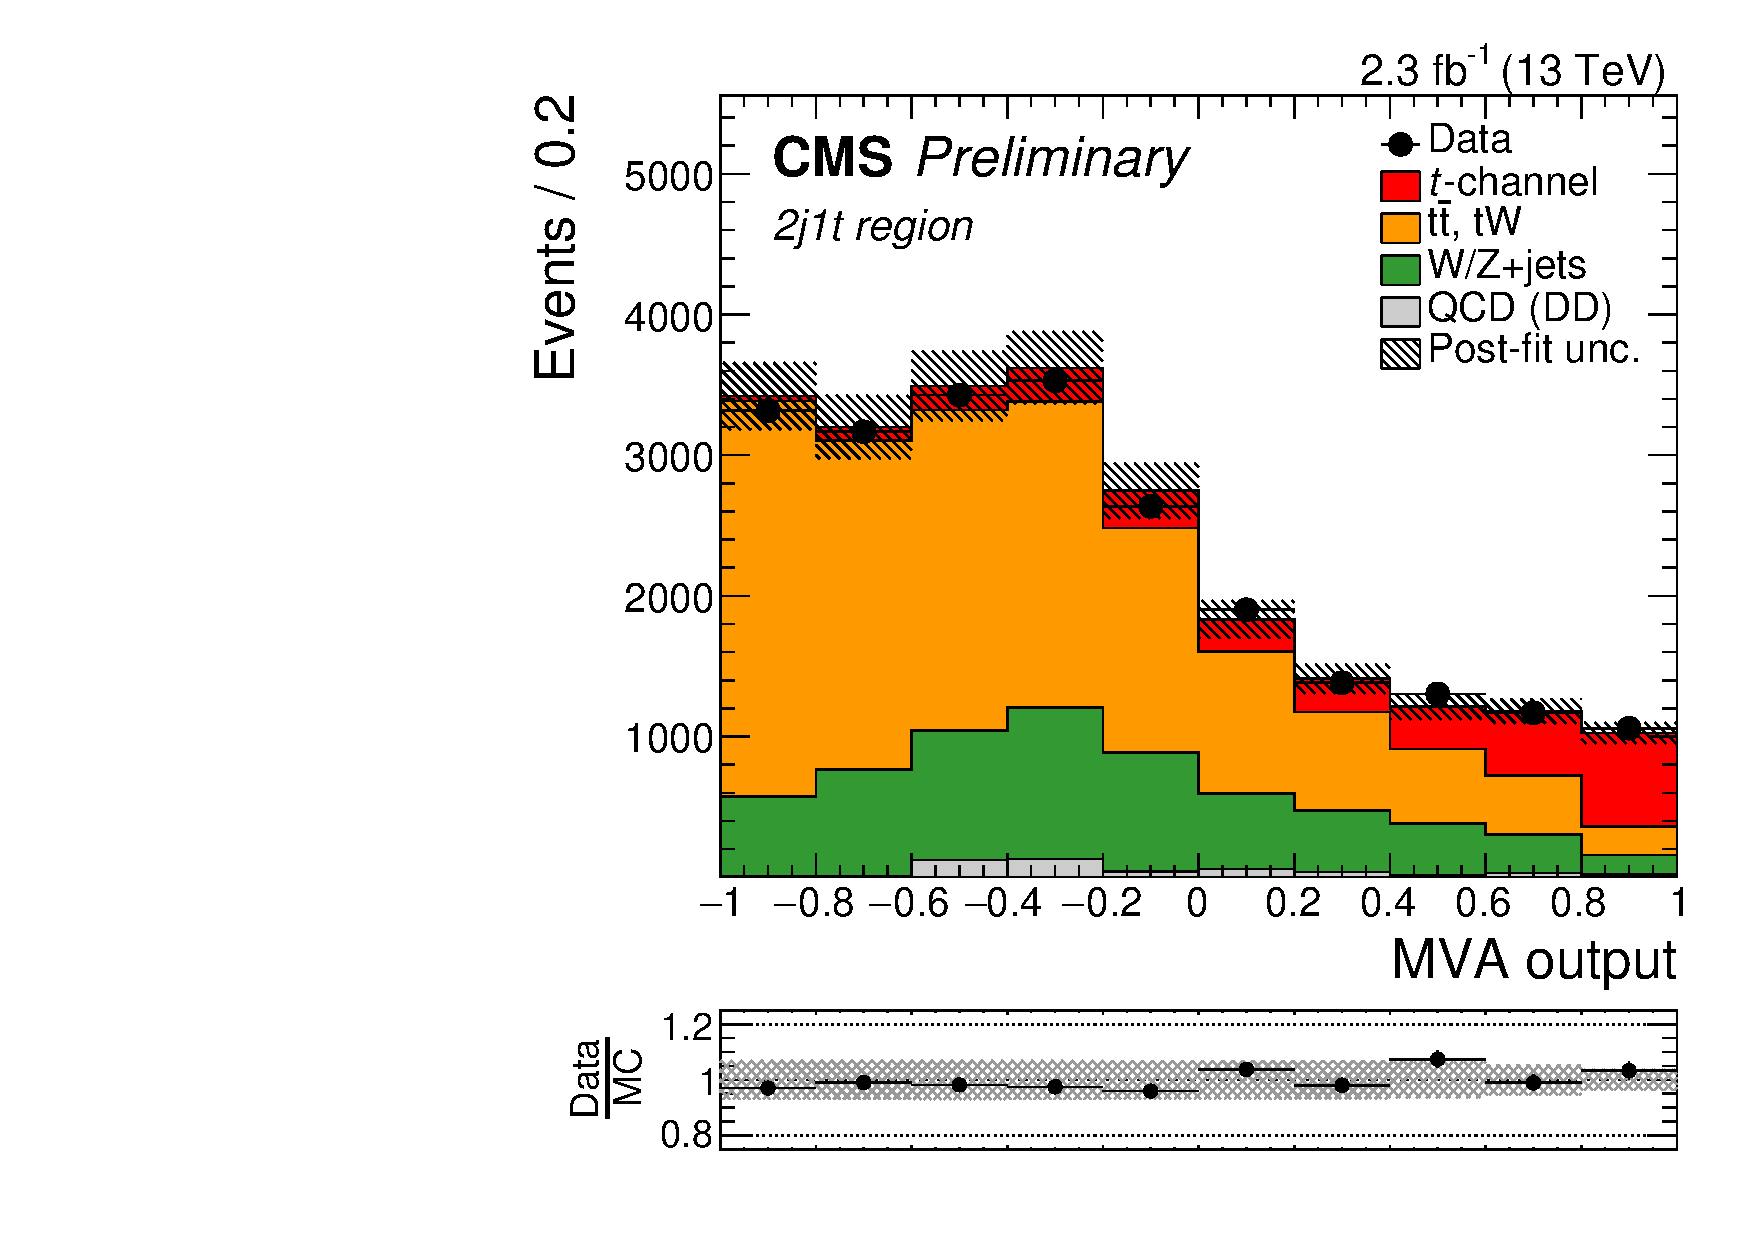
\includegraphics[width=0.4\textwidth]{figures/tchannel/2j1t_BDT.pdf}
\caption{\label{fig:TOP-16-003-2j1t-BDT}Distribution of the BDT discriminant in the signal region. Figure is taken from Ref.~\cite{CMS-PAS-TOP-16-003}.}
\end{center}
\end{figure}



\begin{figure}[htbp]
\begin{center}
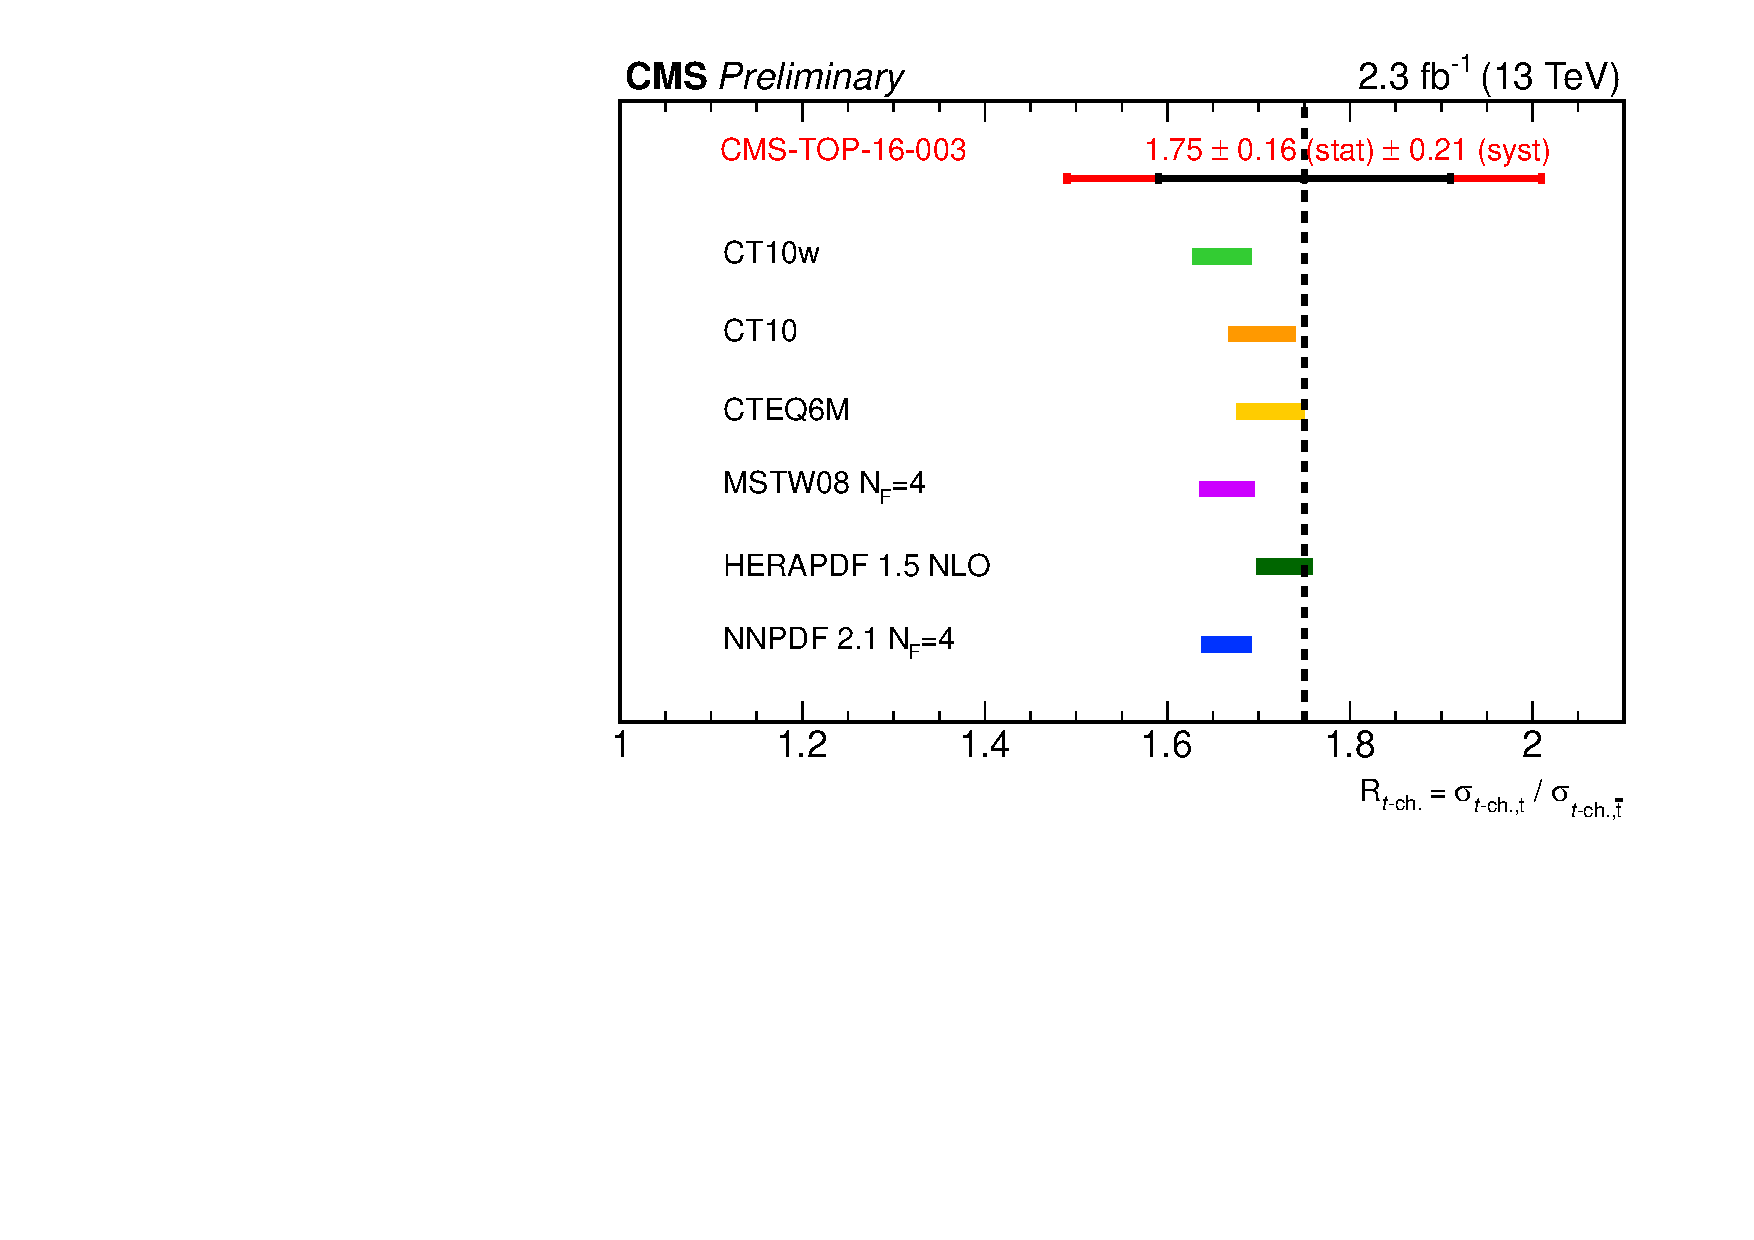
\includegraphics[width=0.7\textwidth]{figures/tchannel/ratio.pdf}
\caption{\label{fig:TOP-16-003-2j1t-R}The cross section ratio of top antiquark over top quark production compared to predictions from various PDF sets. Figure are taken from Ref.~\cite{CMS-PAS-TOP-16-003}}
\end{center}
\end{figure}

The normalized differential cross section as a function of the top quark transverse momentum and rapidity is measured as well. For this, multiple fits are performed to the distributions of \mtw and a Boosted Decision Tree (BDT) discriminant where each fit is restricted to events within an interval of the momentum or rapidity. The estimated signal yields are unfolded to parton level and compared to the predictions by various generators (Fig.~\ref{fig:TOP-16-004-unfolded}). No significant deviation is observed.

\begin{figure}[htbp]
\begin{center}
\parbox[t]{0.49\textwidth}{\centering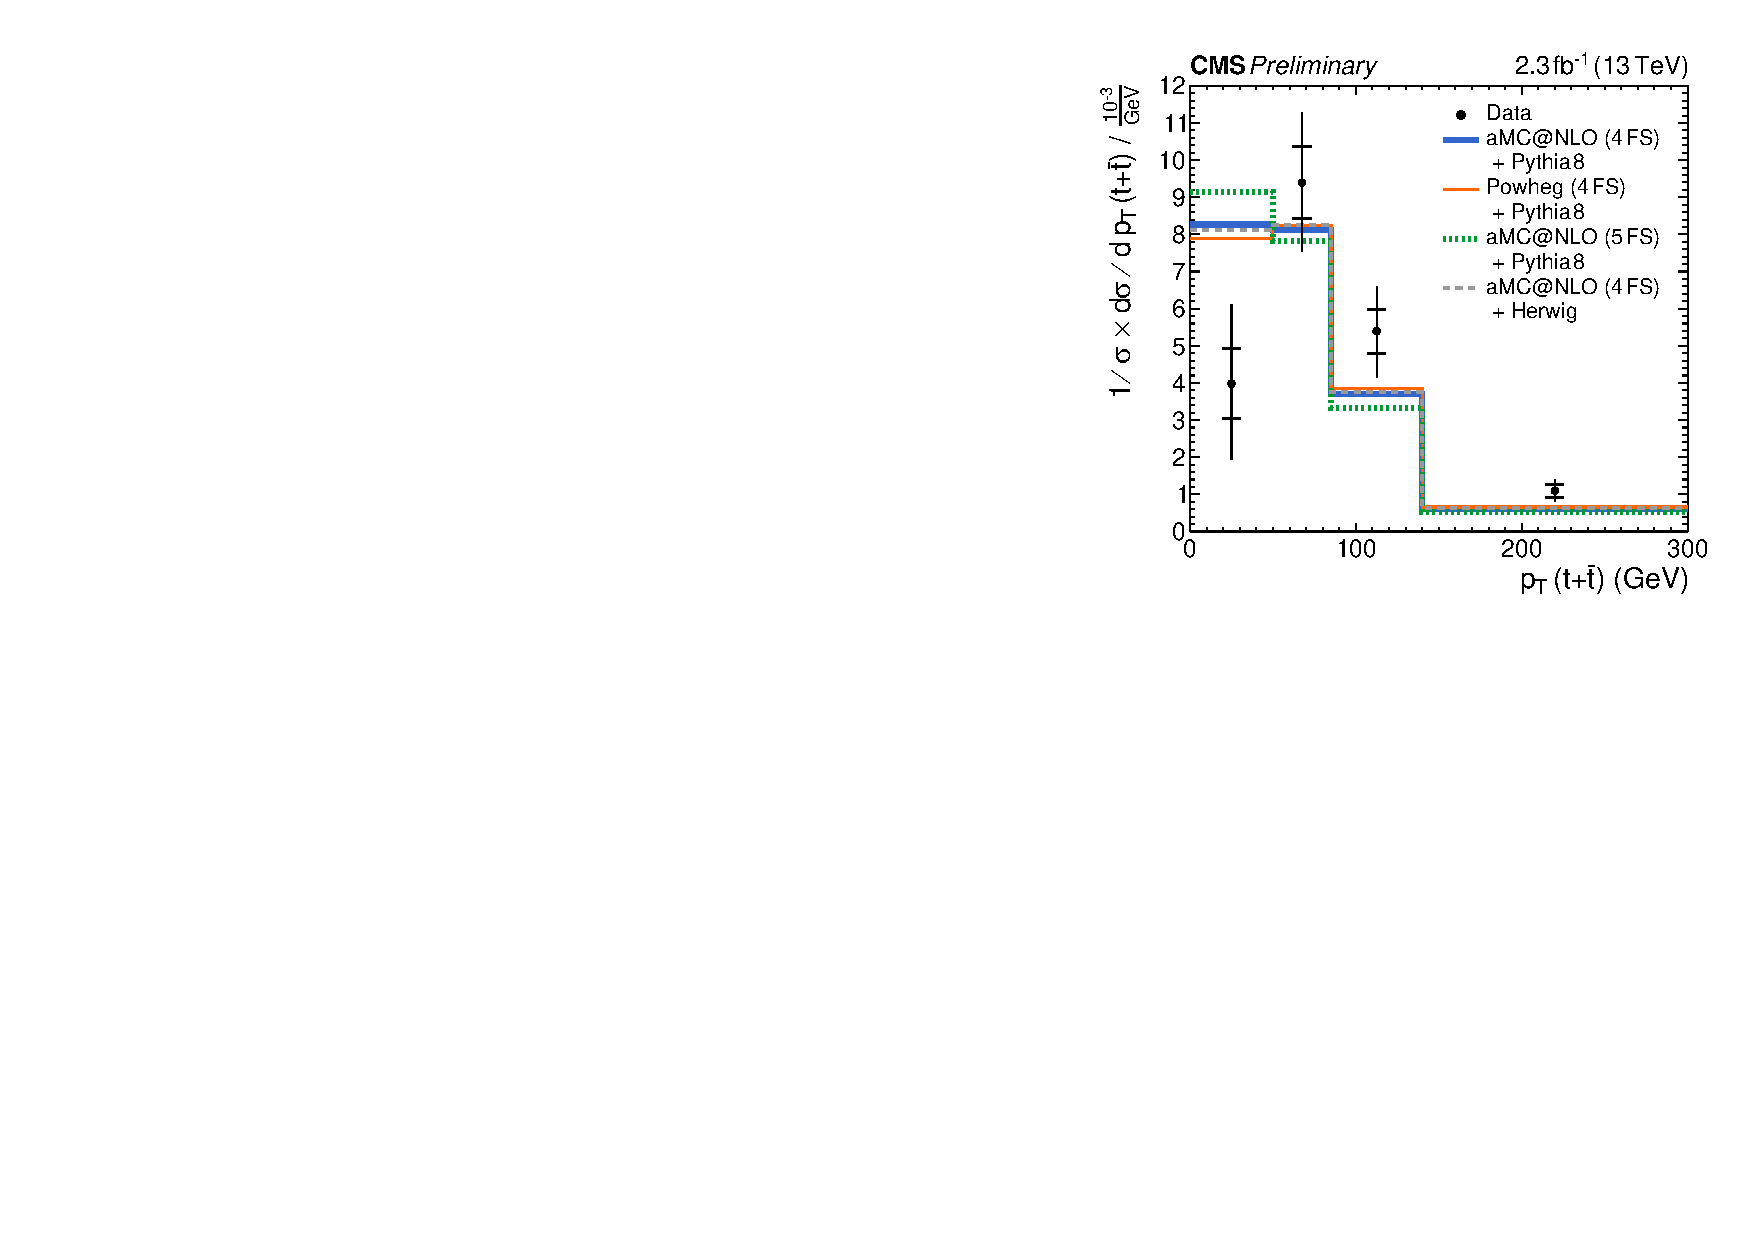
\includegraphics[width=0.42\textwidth]{figures/tchannel_diff/top_pt_unfolded.pdf}\\(a)}
\parbox[t]{0.49\textwidth}{\centering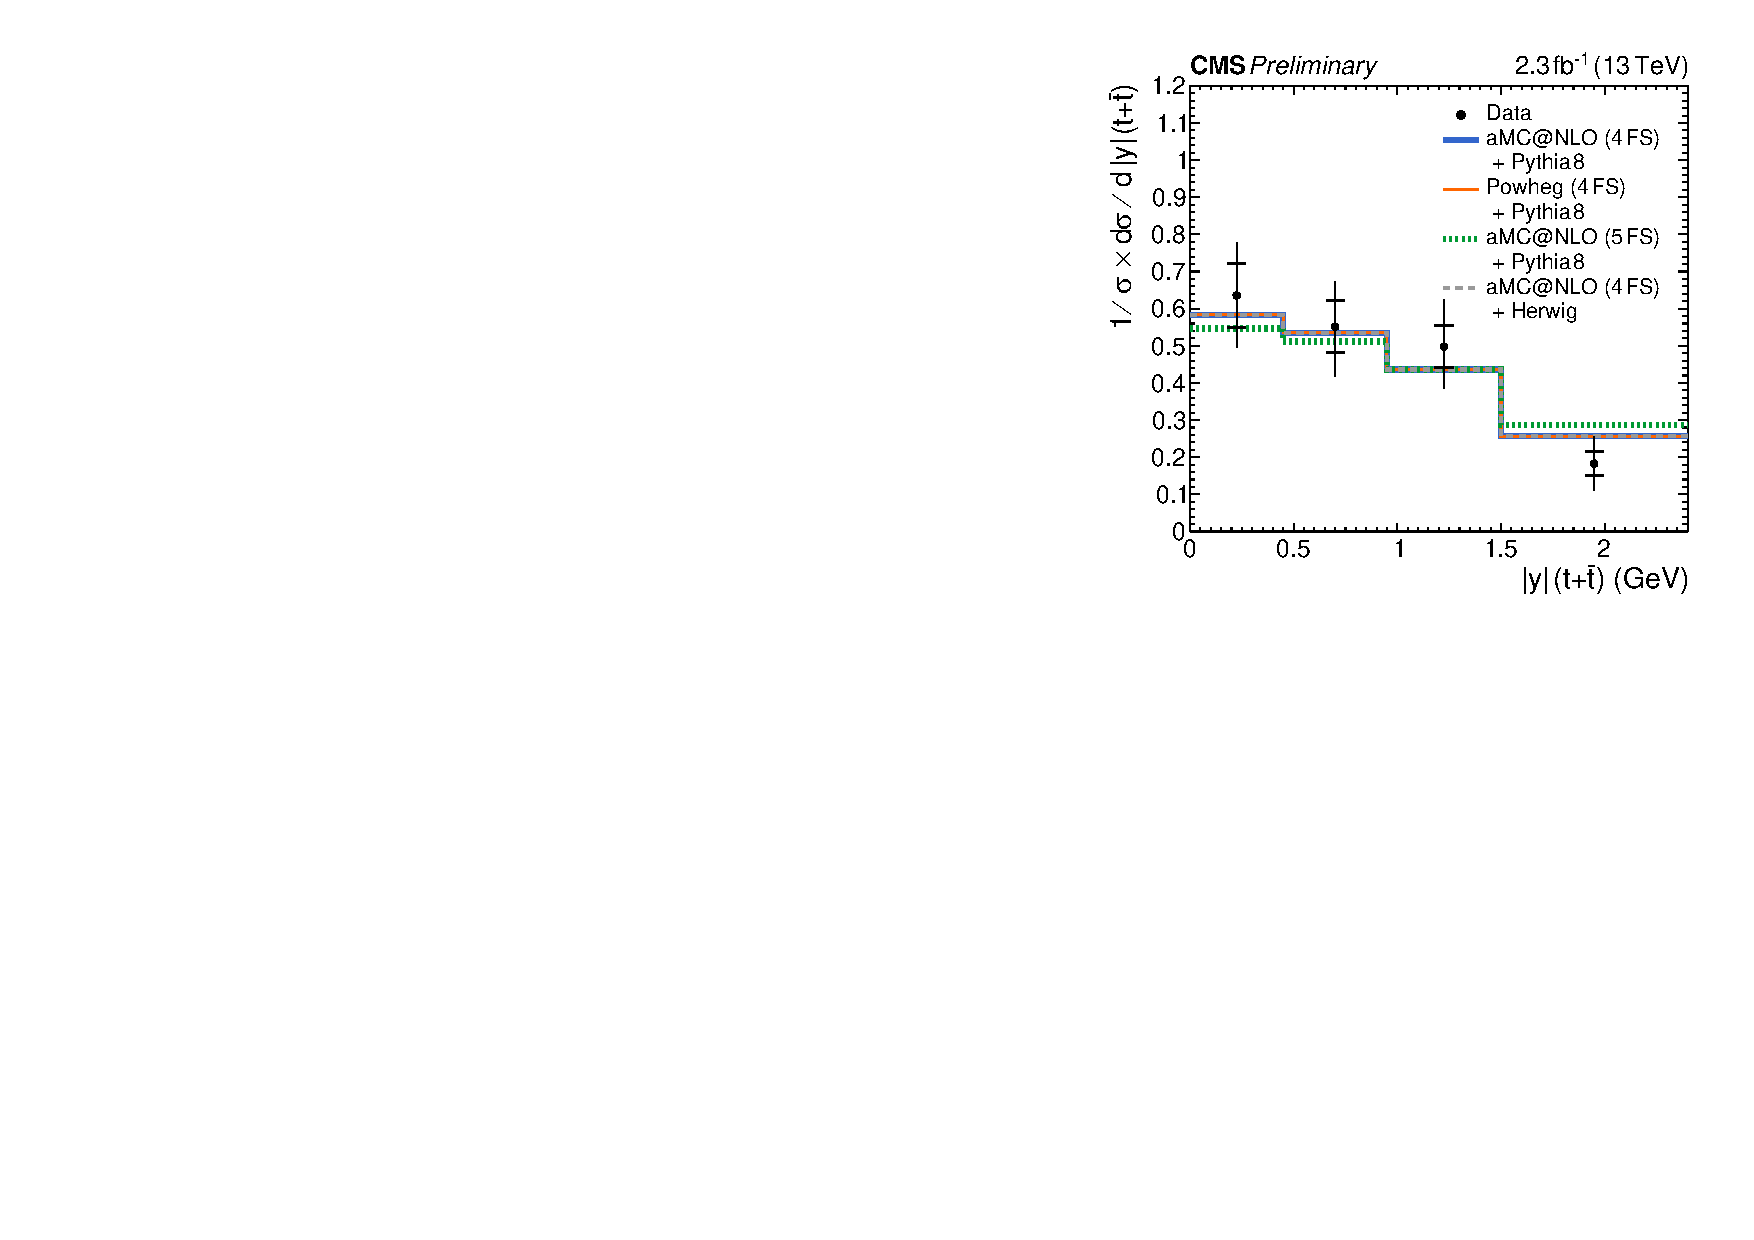
\includegraphics[width=0.42\textwidth]{figures/tchannel_diff/top_y_unfolded.pdf}\\(b)}
\caption{\label{fig:TOP-16-004-unfolded}Normalized differential cross section as a function of (a)~the top quark \pt and (b)~rapidity. Figures are taken from Ref.~\cite{CMS-PAS-TOP-16-004}.}
\end{center}
\end{figure}



\section{Search for $s$-channel single-top-quark production at 7~and 8~TeV}

\begin{figure}[htbp]
\begin{center}
\parbox[t]{0.49\textwidth}{\centering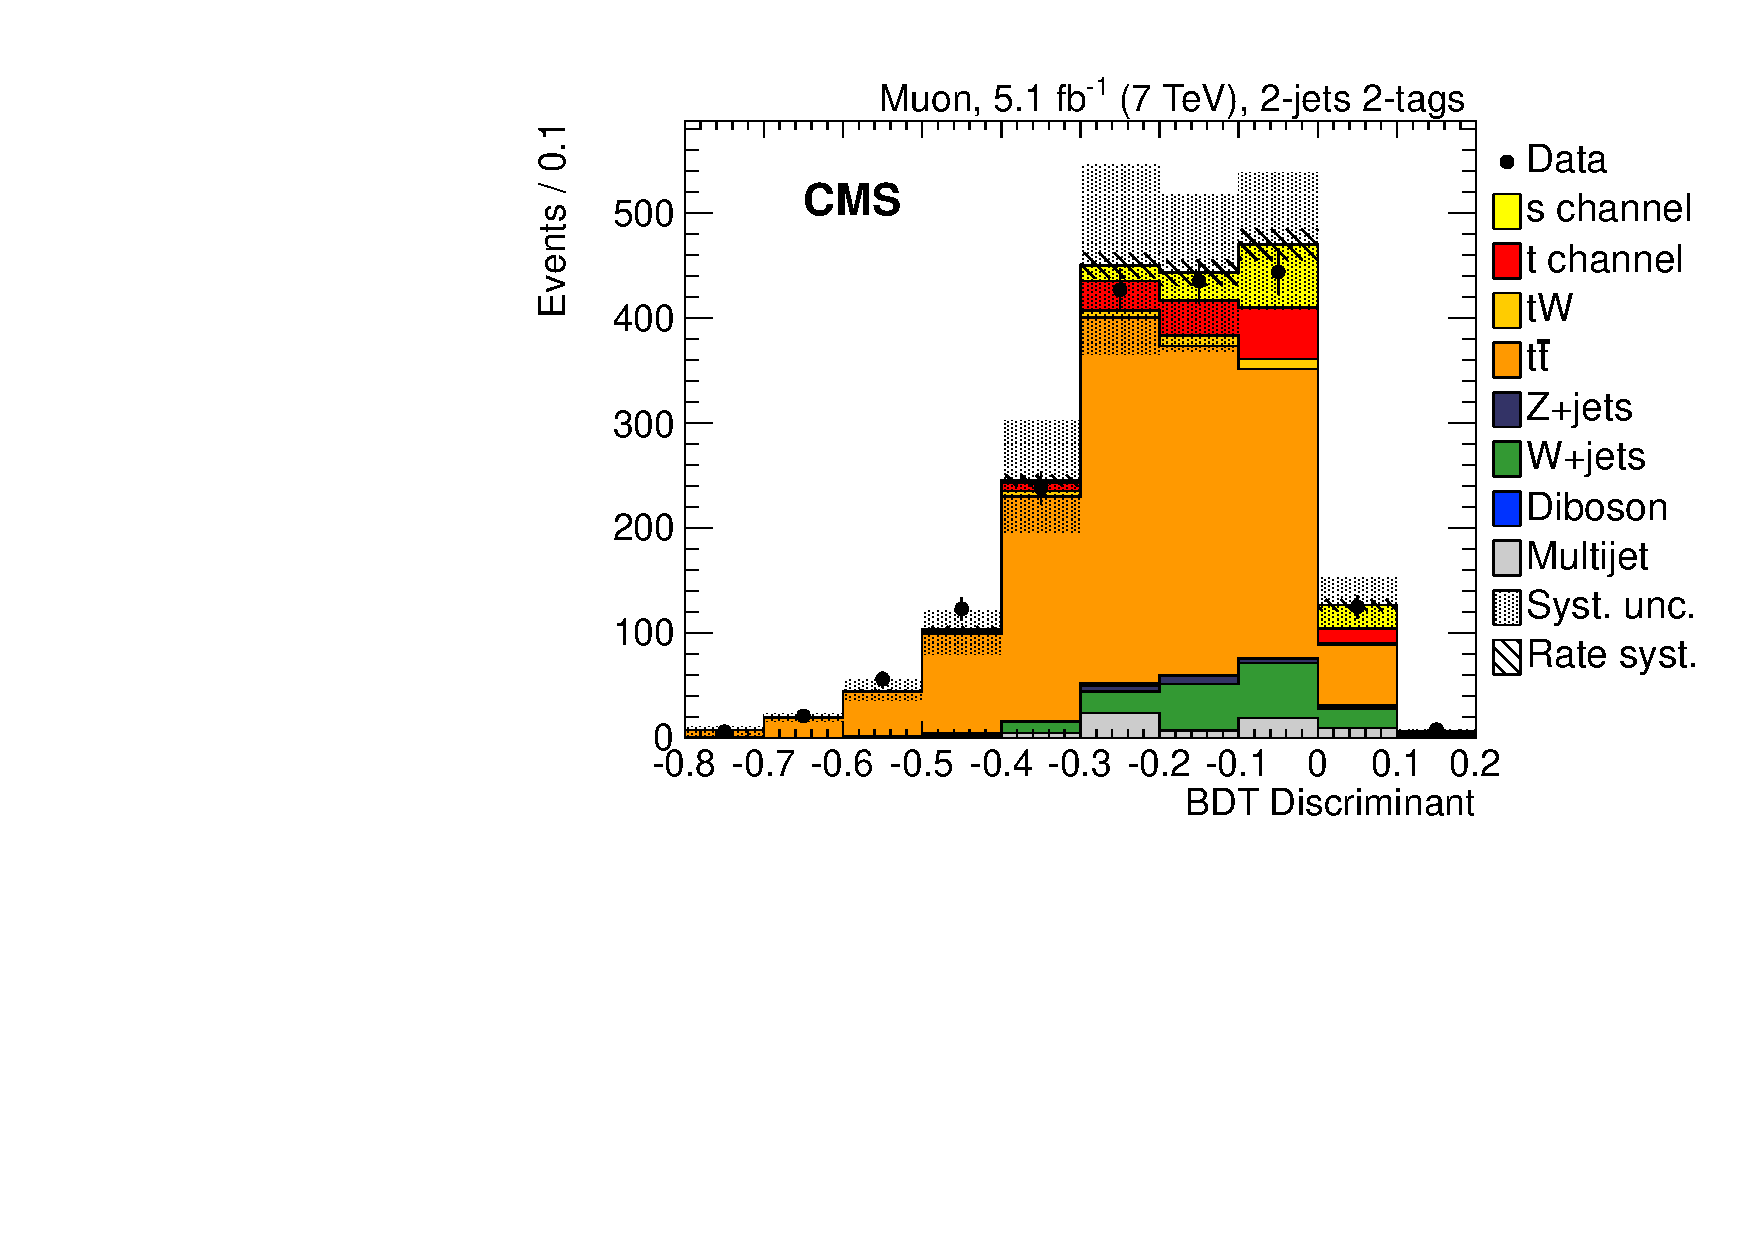
\includegraphics[width=0.48\textwidth]{figures/schannel/mu_7TeV_BDT_signal.pdf}\\(a)}
\parbox[t]{0.49\textwidth}{\centering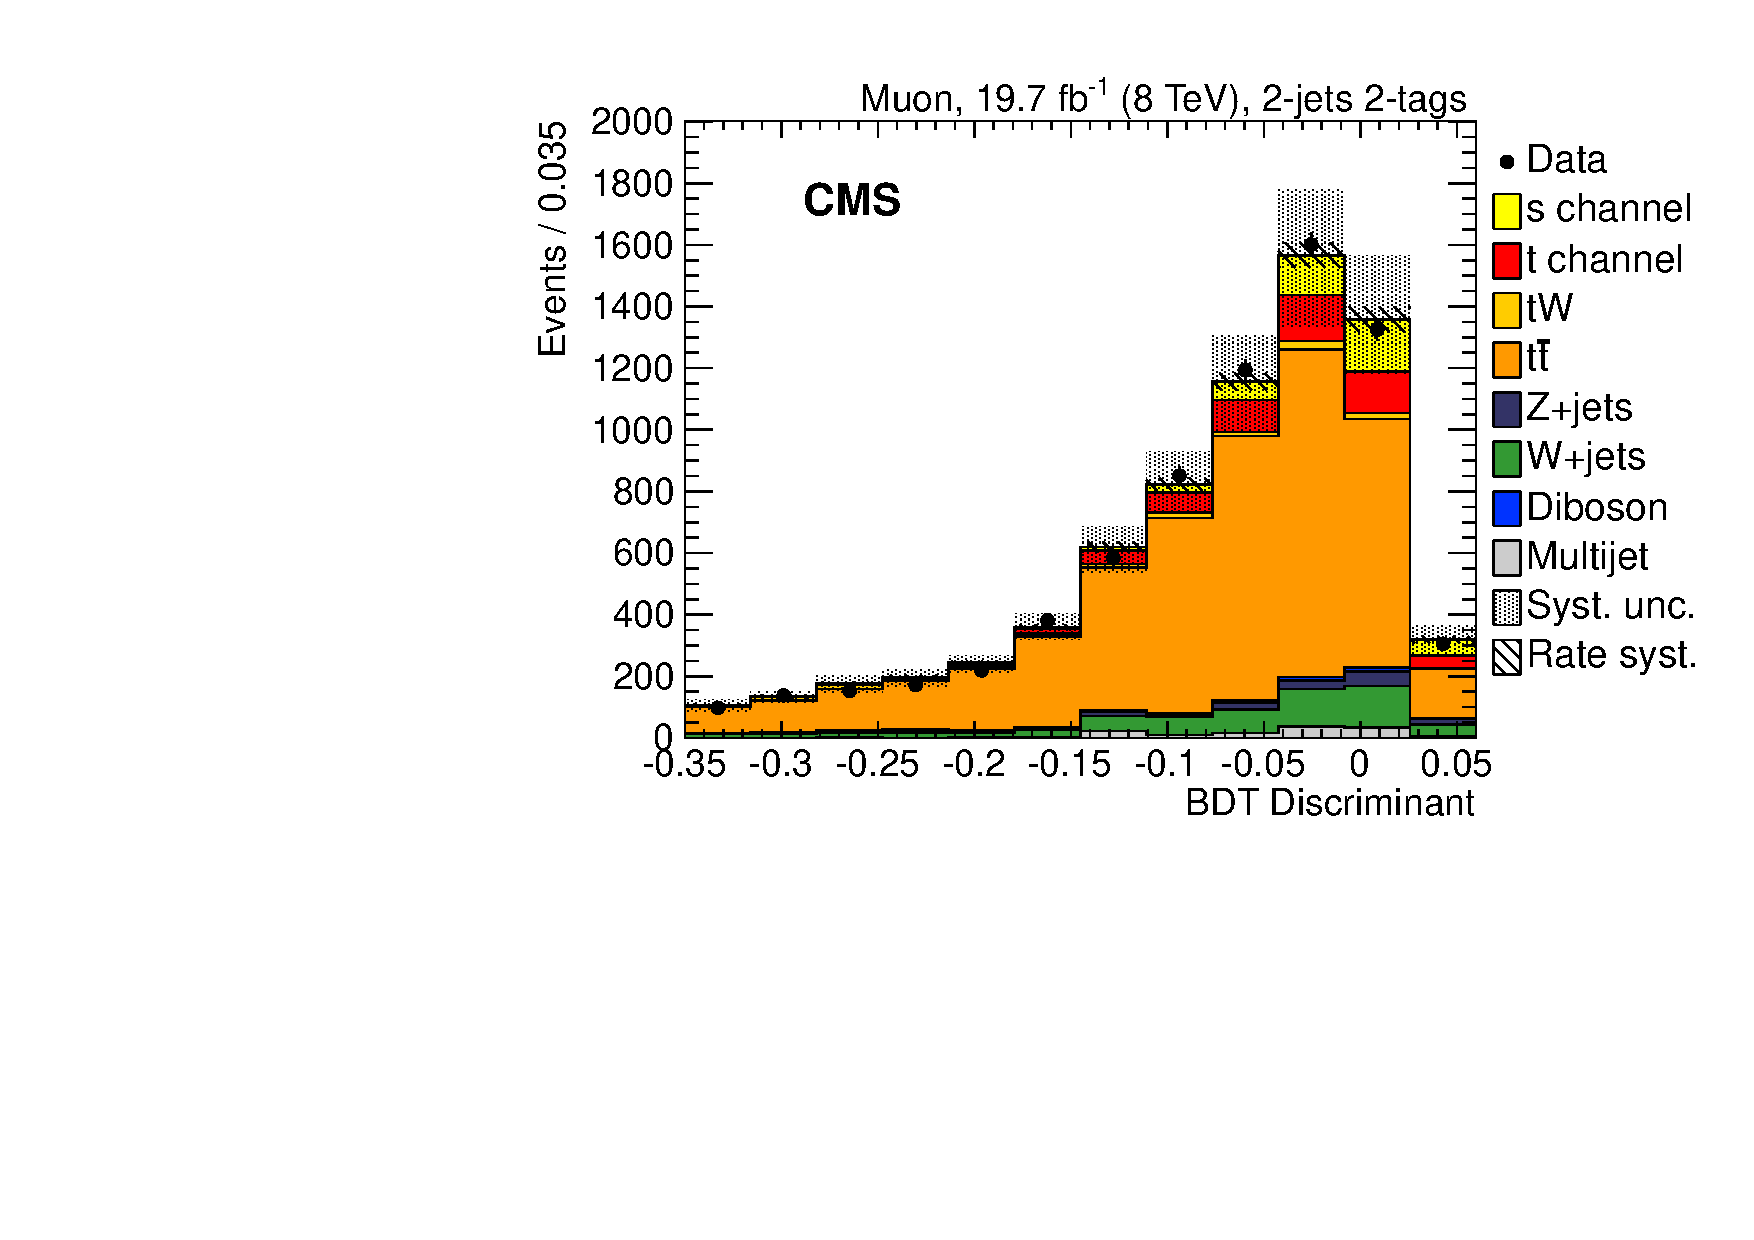
\includegraphics[width=0.48\textwidth]{figures/schannel/mu_8TeV_BDT_signal.pdf}\\(b)}
\caption{Distributions of the BDT discriminant in signal regions: (a)~7~TeV; (b)~8~TeV. Figures are taken from Ref.~\cite{CMS-PAS-TOP-13-009}}
\end{center}
\end{figure}

\section{Measurement of $t$-channel single-top-quark polarisation}

\begin{figure}[htbp]
\begin{center}
\parbox[t]{0.55\textwidth}{\centering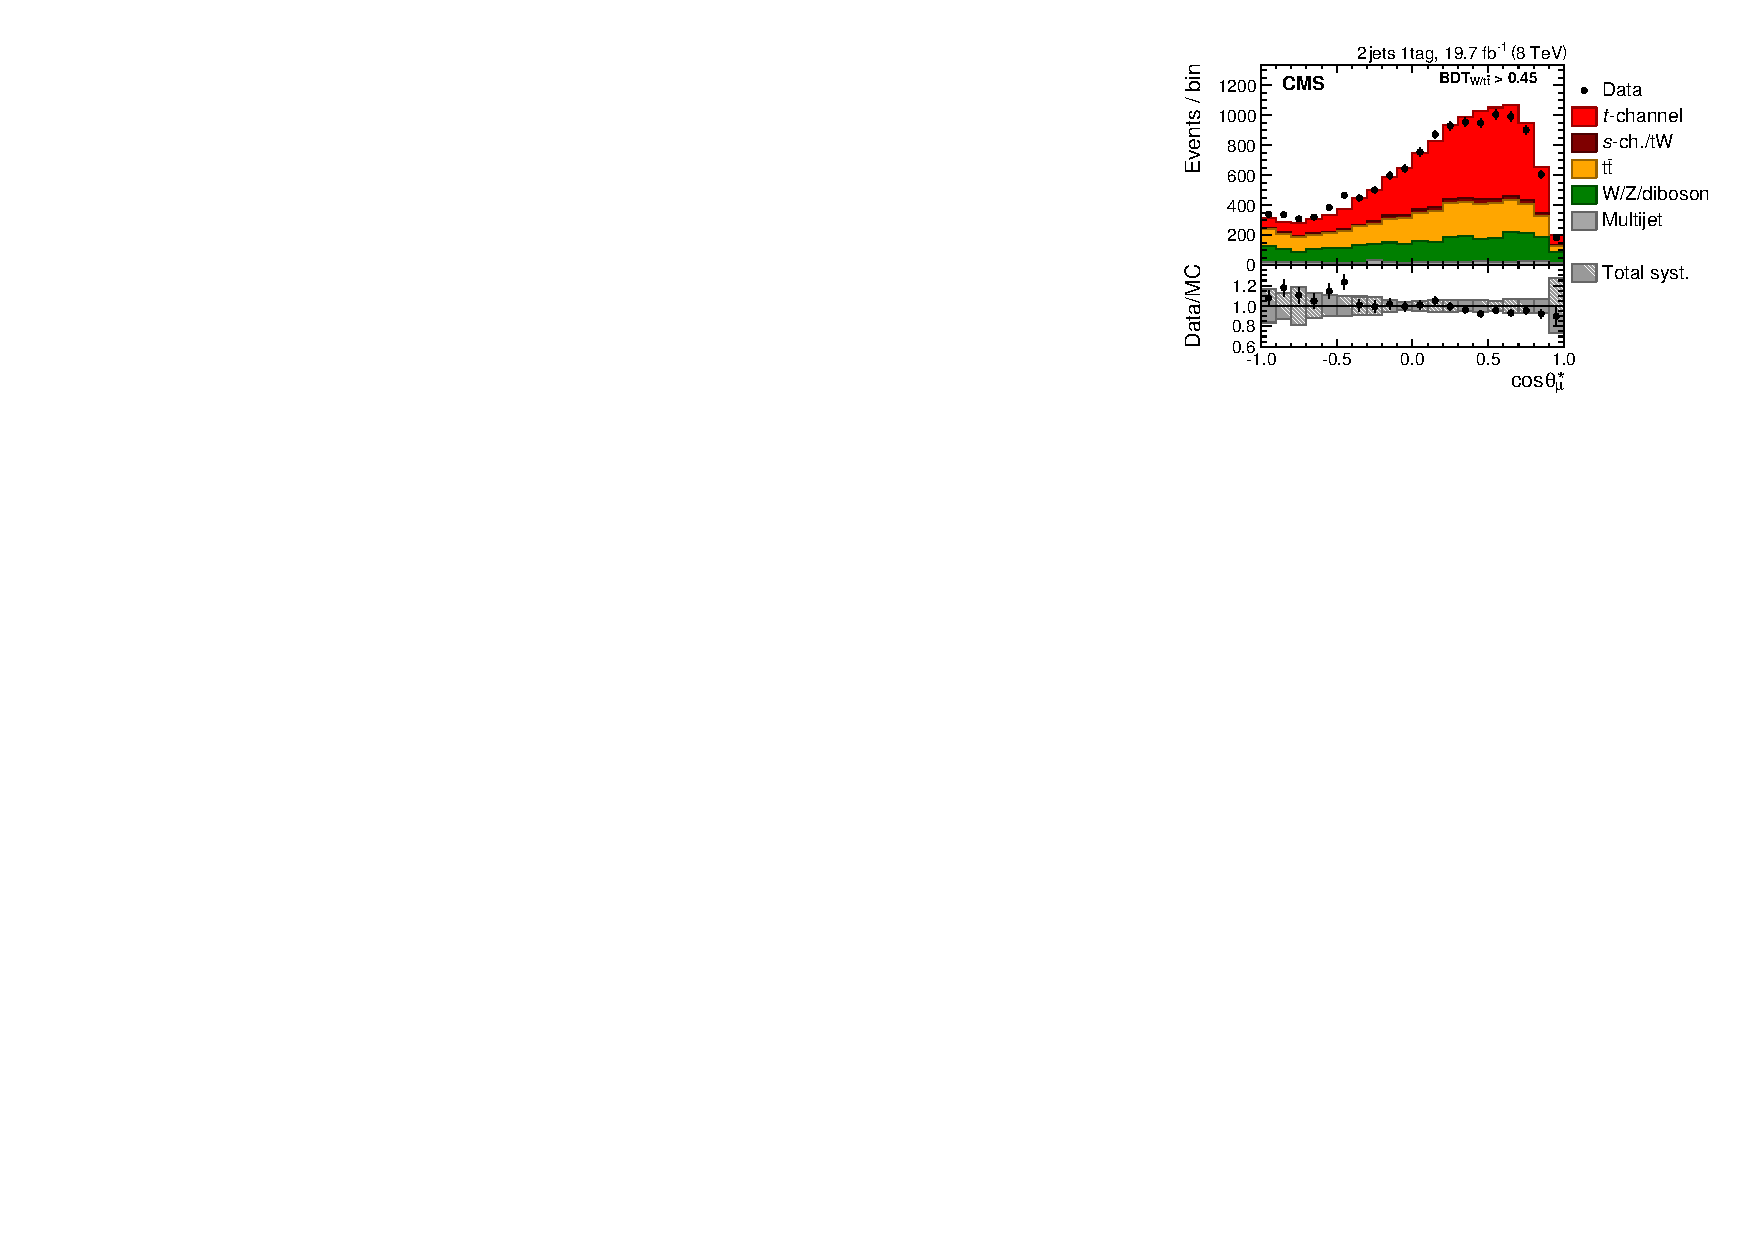
\includegraphics[width=0.54\textwidth]{figures/polarization/2j1t_cos_theta.pdf}\\(a)}
\parbox[t]{0.44\textwidth}{\centering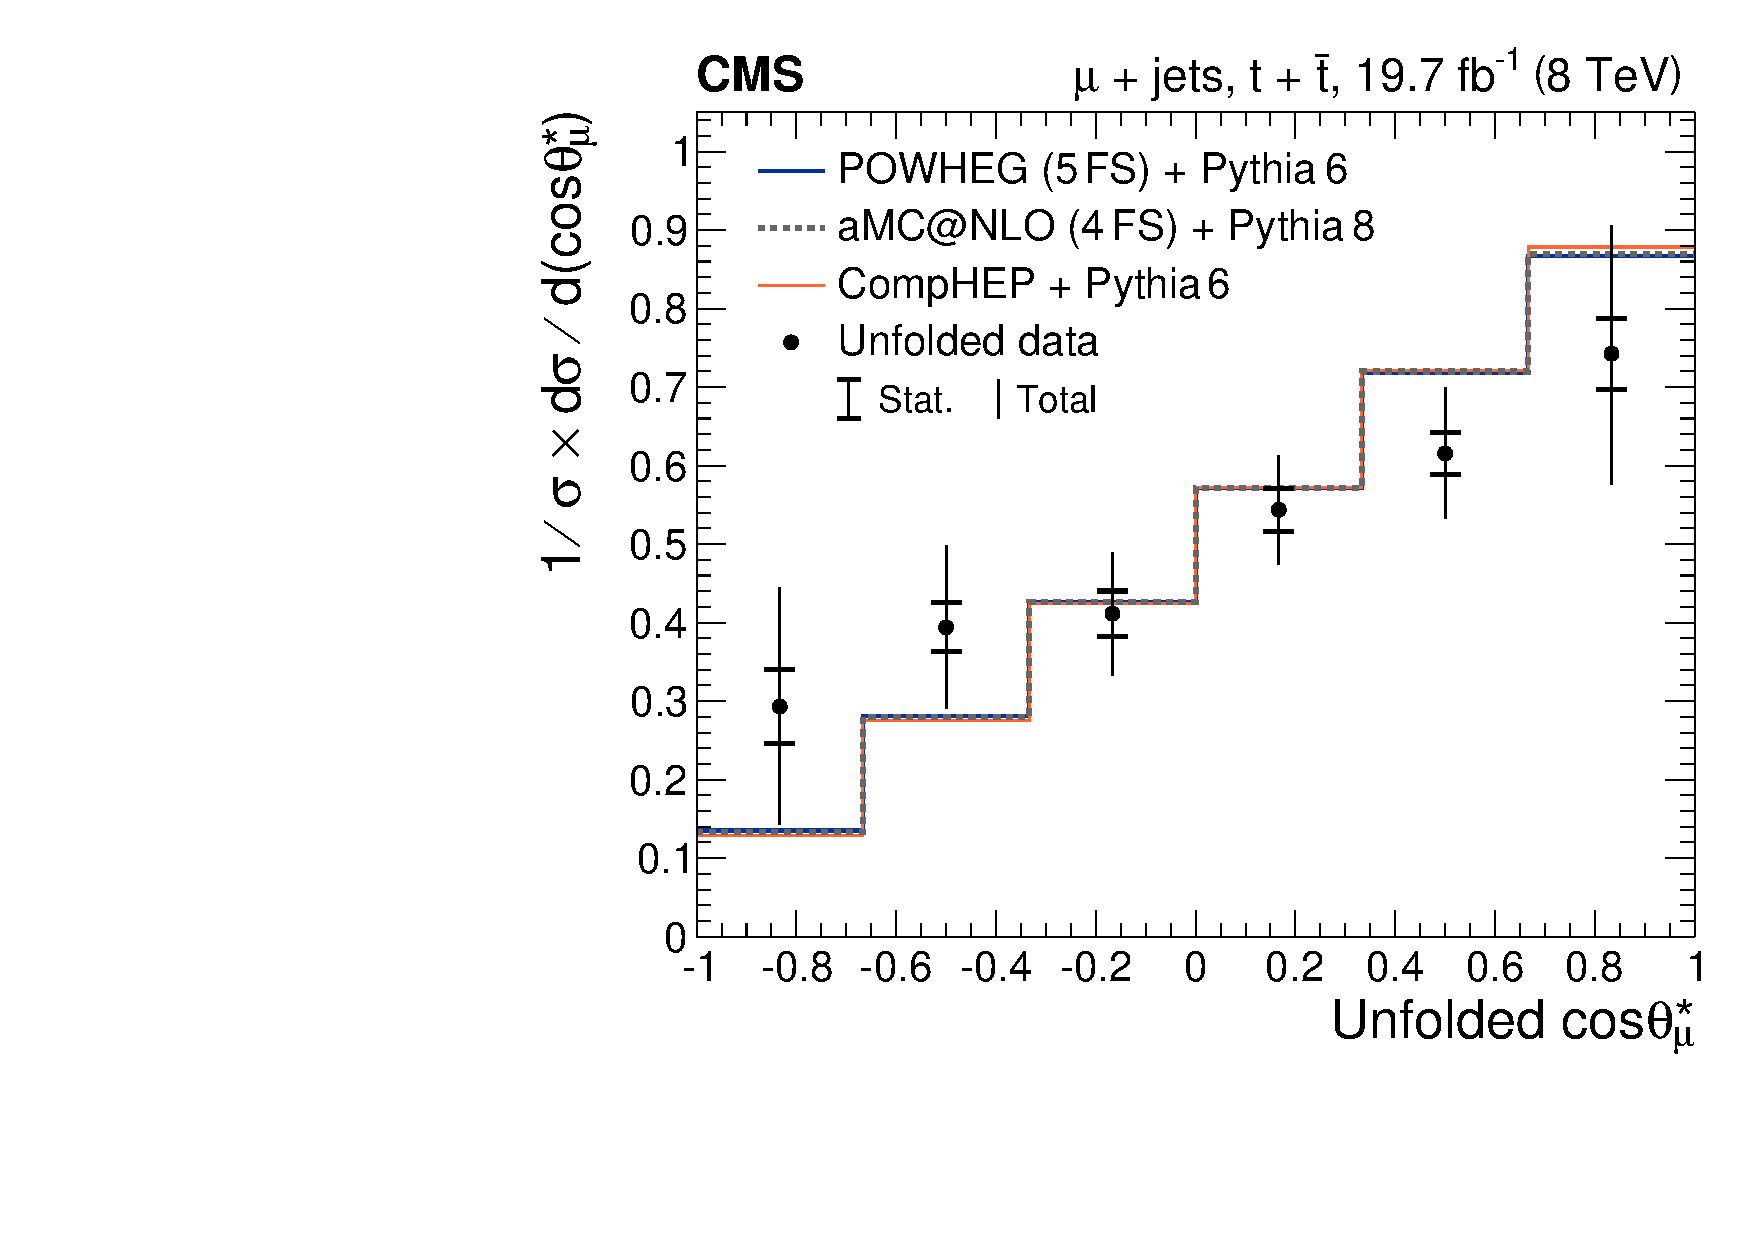
\includegraphics[width=0.43\textwidth]{figures/polarization/cos_theta_unfolded.pdf}\\(b)}
\caption{Distributions of the (a)~reconstructed and (b)~unfolded polarisation angle. Figures are taken from Ref.~\cite{CMS-PAS-TOP-13-001}}
\end{center}
\end{figure}


\section{Search for flavour changing neutral currents involing photons}

\begin{figure}[htbp]
\begin{center}
\parbox[t]{0.49\textwidth}{\centering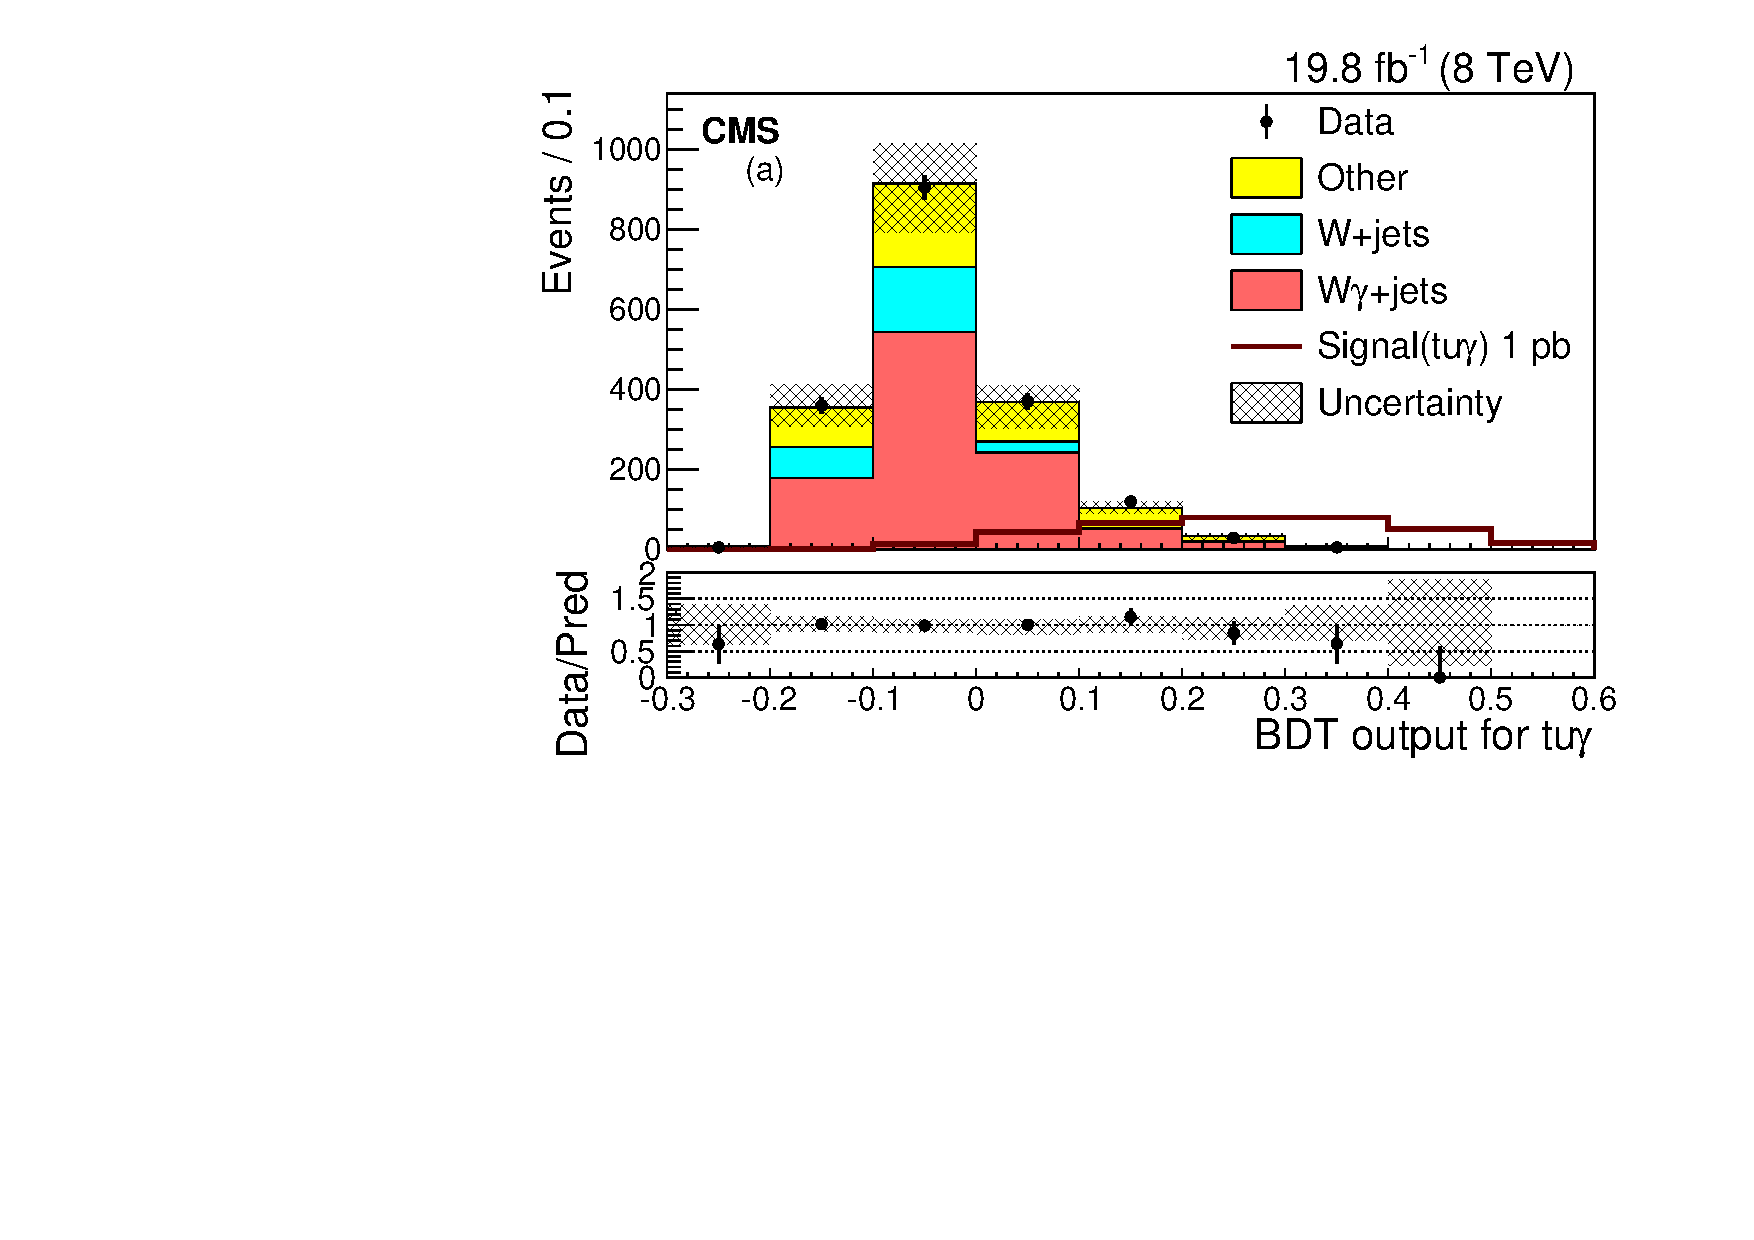
\includegraphics[width=0.48\textwidth]{figures/FCNC/BDT_utg.pdf}\\(a)}
\parbox[t]{0.49\textwidth}{\centering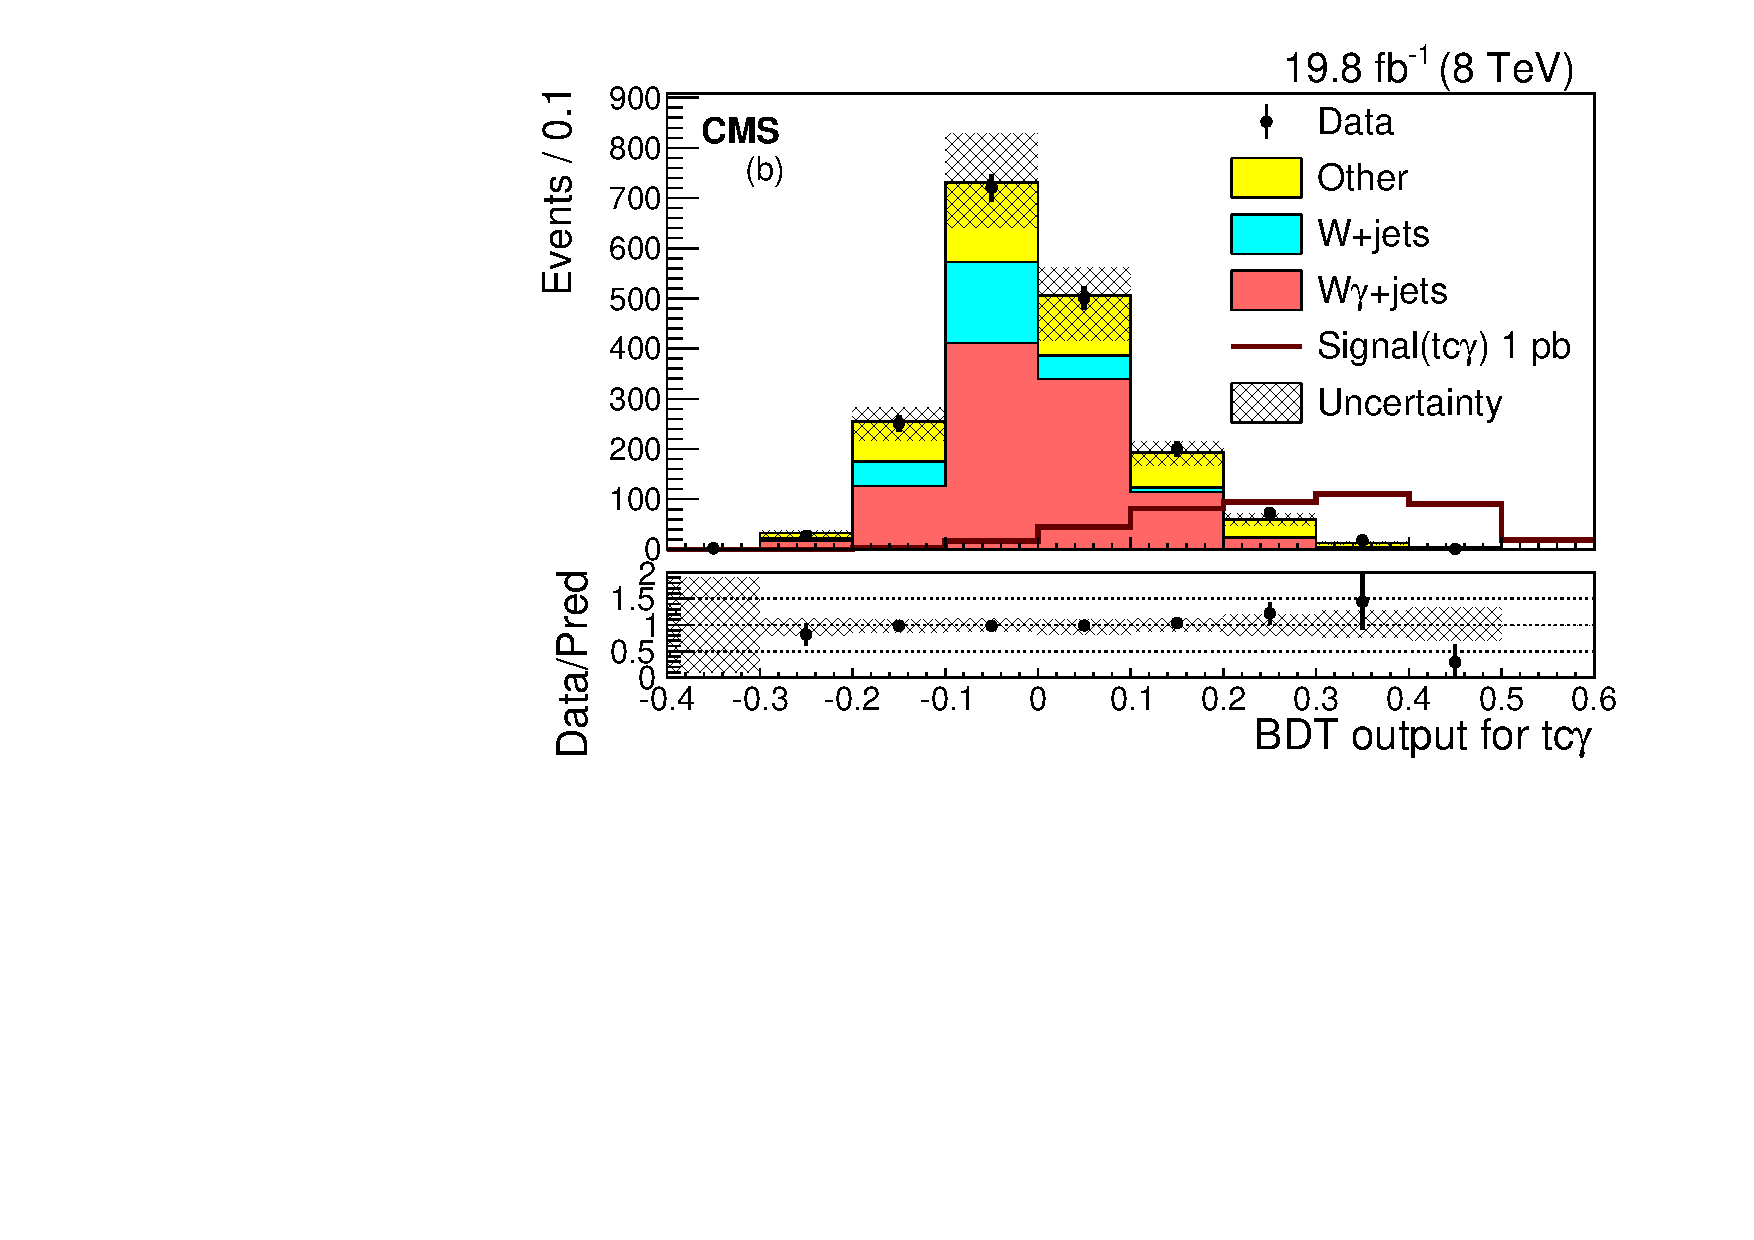
\includegraphics[width=0.48\textwidth]{figures/FCNC/BDT_ctg.pdf}\\(b)}
\caption{Distributions of the FCNC BDT discriminants: (a)~$\mathrm{tu}\gamma$-, (b)~$\mathrm{tc}\gamma$-vertex. Figures are taken from Ref.~\cite{CMS-PAS-TOP-14-003}.}
\end{center}
\end{figure}

\begin{figure}[htbp]
\begin{center}
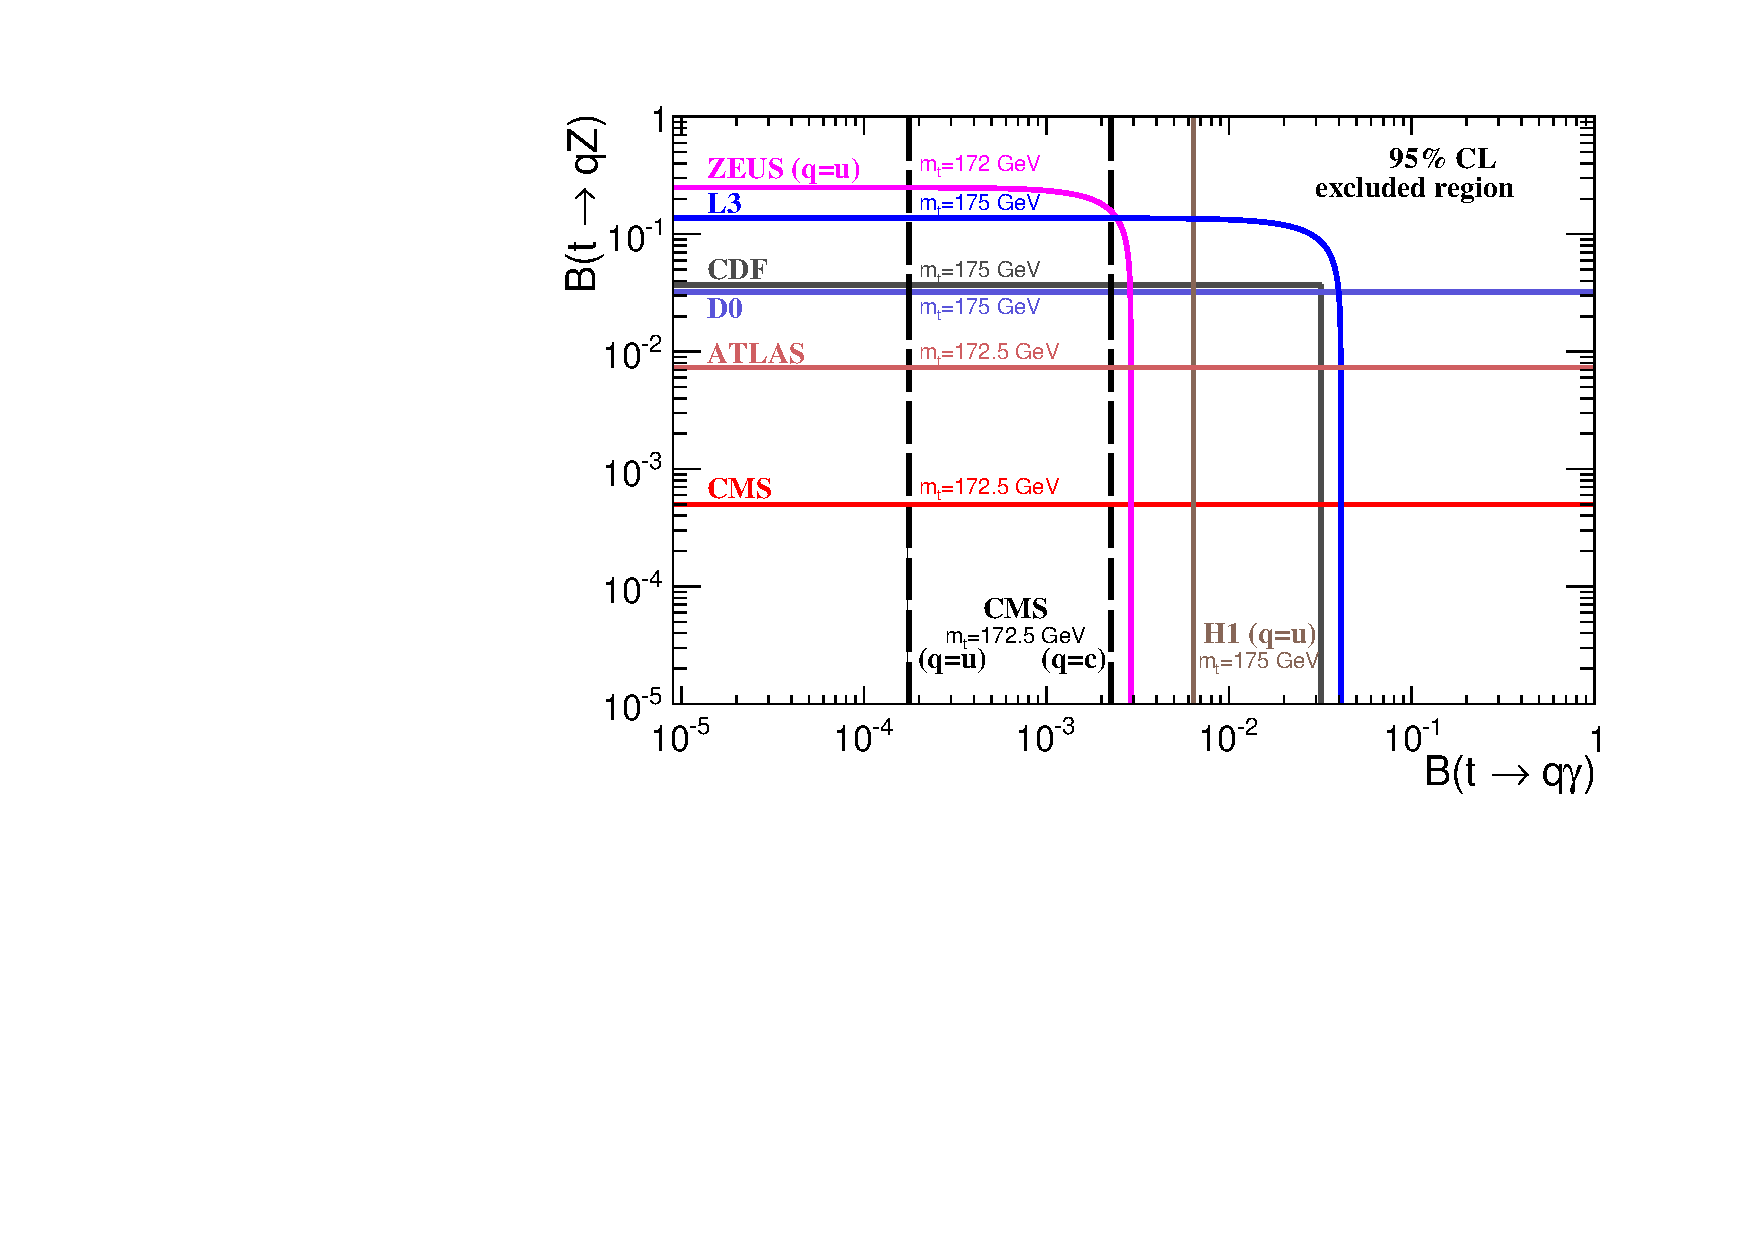
\includegraphics[width=0.7\textwidth]{figures/limits.pdf}
\caption{Overview of limits on FCNC $\mathrm{t}\to\mathrm{q}\gamma$ and $\mathrm{t}\to\mathrm{qZ}$ branching ratios from various experimemts. Figure is taken from Ref.~\cite{CMS-PAS-TOP-14-003}.}
\end{center}
\end{figure}

\section{Conclusion}

\begin{figure}[htbp]
\begin{center}
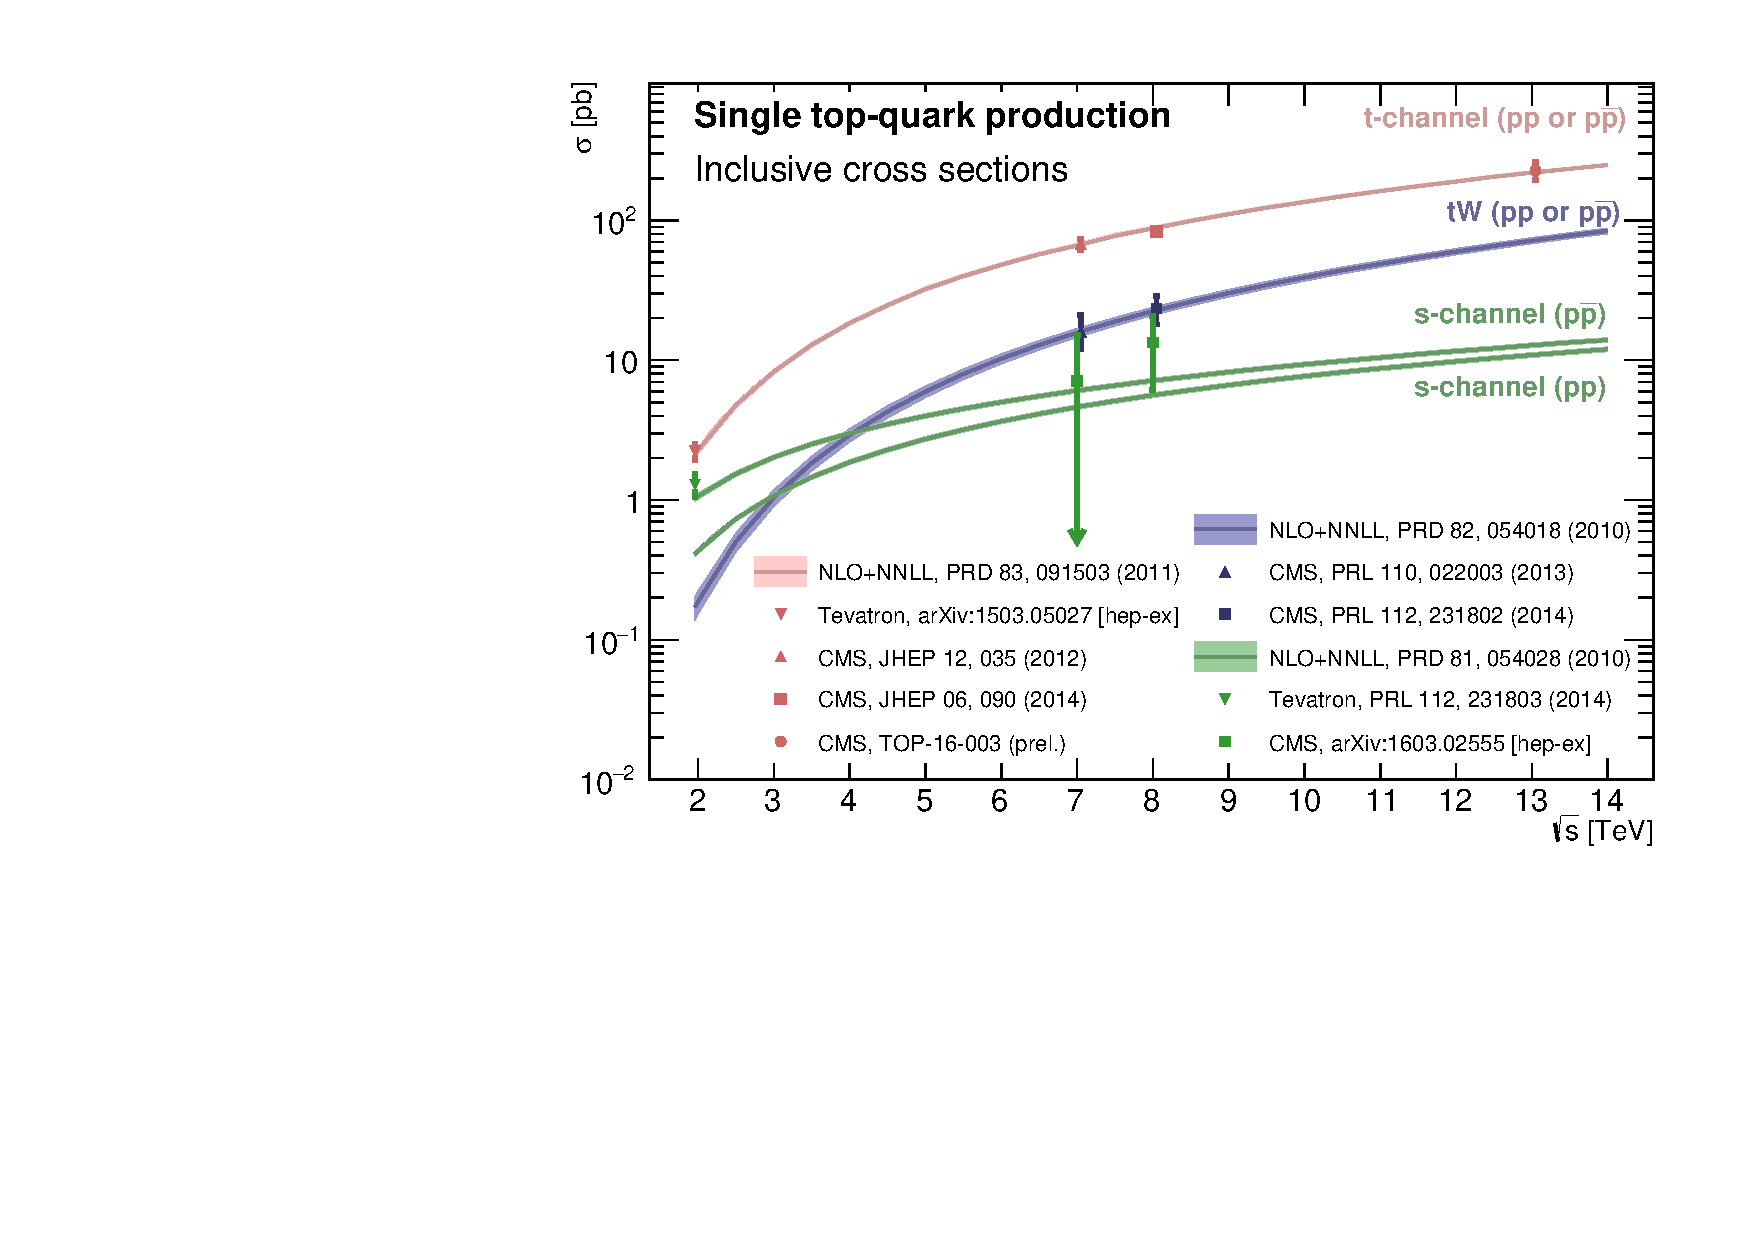
\includegraphics[width=0.7\textwidth]{figures/singletop_sqrts.pdf}
\caption{Overview of single-top-quark cross section measurements for $t$-, tW-, and $s$-channel by the CMS collaboration at various LHC energies.}
\end{center}
\end{figure}

\clearpage

\begin{thebibliography}{99}

\bibitem{CMS-PAS-TOP-16-003}{CMS Collaboration, \emph{Measurement of the inclusive cross section of single top-quark production in the $t$-channel at 13~TeV}, CMS Physics Analysis Summary CMS-PAS-TOP-16-003, 2016.}

\bibitem{CMS-PAS-TOP-16-004}{CMS Collaboration, \emph{Measurement of the differential cross section for t-channel single-top-quark production at $\sqrt{\mathrm{s}}=13~\mathrm{TeV}$}, CMS Physics Analysis Summary CMS-PAS-TOP-16-004, 2016.}

\bibitem{CMS-PAS-TOP-13-009}{CMS Collaboration, \emph{Search for $s$ channel single top quark production in pp collisions at $\sqrt{s}$~=~7~and 8~TeV}, submitted to \emph{JHEP}, {\tt arXiv:1603.02555\,[hep-ex]}, 2016.}

\bibitem{CMS-PAS-TOP-13-001}{CMS Collaboration, \emph{Measurement of top quark polarisation in t-channel single top quark production}, \emph{JHEP} \textbf{04} (2016) 073, {\tt arXiv:1511.02138\,[hep-ex]}, 2016.}

\bibitem{CMS-PAS-TOP-14-003}{CMS Collaboration, \emph{Search for anomalous single top quark production in association with a photon in pp collisions at $\sqrt{s}=8~\mathrm{TeV}$}, \emph{JHEP} \textbf{04} (2016) 035, {\tt arXiv:1511.03951\,[hep-ex]}, 2016.}

\end{thebibliography}

\end{document}
